%!Tex program = xelatex
\documentclass[11pt,openany]{book}              % Book class in 11 points

%\documentclass[justified,twoside]{tufte-book}
%\usepackage[UTF8]{ctex}


\parindent0pt  \parskip10pt             % make block paragraphs
%\raggedright                            % do not right justify
\usepackage{xcolor}
\usepackage{amsmath}
\usepackage{amssymb}
\usepackage{bm}
\usepackage[round]{natbib}
\usepackage{graphicx}
\usepackage{subfigure}
\usepackage{amsthm}
\usepackage{tgpagella}
\usepackage{enumerate}
\usepackage{emptypage}
\usepackage{multirow}
\usepackage{booktabs}
\usepackage{braket}
\usepackage[LGR,T1]{fontenc}
\newcommand{\textgreek}[1]{\begingroup\fontencoding{LGR}\selectfont#1\endgroup}
\usepackage{lipsum}
\usepackage{tcolorbox}
%\usepackage{hyperref}
 \usepackage{pgfplots}
 \pgfplotsset{compat=newest}
  %% the following commands are needed for some matlab2tikz features
  \usetikzlibrary{plotmarks}
  \usetikzlibrary{arrows.meta}
  \usepgfplotslibrary{patchplots}
  \usepackage{grffile}


  %% you may also want the following commands
  %\pgfplotsset{plot coordinates/math parser=false}
  %\newlength\figureheight
  %\newlength\figurewidth

\usepackage{microtype}


\definecolor{echodrk}{HTML}{0099cc}
\definecolor{mymauve}{rgb}{0.58,0,0.82}
\usepackage[colorlinks,linkcolor=mymauve,citecolor=echodrk]{hyperref}

\usepackage{cleveref}
\definecolor{boxgray}{rgb}{0.9,0.9,0.9}
\definecolor{boxpink}{rgb}{0.9,0.7,0.7}

\renewcommand\vec{\mathbf}
\newcommand\mat{\mathbf}

\makeatletter
\renewcommand{\thesection}{%
	\ifnum\c@chapter<1 \@arabic\c@section
	\else \thechapter.\@arabic\c@section
	\fi
}
\makeatother



\usepackage{marginnote}
\renewcommand*{\marginfont}{\footnotesize}
\newcommand{\joan}[1]{{\color{green}#1}}
\newcommand{\michael}[1]{{\color{magenta}#1}} \newcommand{\taco}[1]{{\color{blue}#1}}
\newcommand{\petar}[1]{{\color{cyan}#1}}


\definecolor{olivegreen}{HTML}{006400}
\definecolor{echoblue}{HTML}{0099CC}
\definecolor{gold}{HTML}{F09A00}
\definecolor{vividred}{HTML}{E60B42}
\definecolor{echonavy}{HTML}{0054B2}
\definecolor{darkgry}{HTML}{333333}
\definecolor{echopurple}{HTML}{9400D1}
\usepackage{tikz}
\tikzset{every picture/.style={line width=0.75pt}} %set default line width to 0.75pt    


\newcommand*{\horzbar}{\rule[.5ex]{2.5ex}{0.5pt}}


\newtheoremstyle{break}
{\topsep}{\topsep}%
{\itshape}{}%
{\bfseries}{}%
{\newline}{}%
%\theoremstyle{break}

\newtheorem{definition}{Definition}
\newtheorem{theorem}{Theorem}
\newtheorem{remark}{Remark}
\newtheorem{example}{Example}
\newtheorem{corollary}{Corollary}
\newtheorem{consequence}{Consequence}
\newtheorem{conjecture}{Conjecture}
\newcommand{\sign}{{\rm sign}}
\newcommand{\argmin}{\mathop{\rm argmin}}
\newcommand{\argmax}{\mathop{\rm argmax}}
\newcommand{\tr}{\mathop{\rm tr}}
\newcommand{\dd}{{\rm d}}

\usepackage{fancyhdr}

\fancypagestyle{plain}{ %
	\fancyhf{} % remove everything
	\renewcommand{\headrulewidth}{0pt} % remove lines as well
	\renewcommand{\footrulewidth}{0pt}
}


\fancypagestyle{fancybook}{%
	\fancyhf{}%
	% Note the ## here. It's required because \fancypagestyle is making a macro (\ps@fancybook).
	% If we just wrote #1, TeX would think that it's the argument to \ps@fancybook, but
	% \ps@fancybook doesn't take any arguments, so TeX would complain with an error message.
	% You are not expected to understand this.
	\renewcommand*{\sectionmark}[1]{ \markright{\thesection\ ##1} }%
	%\renewcommand*{\chaptermark}[1]{ \markboth{\chaptername\ \thechapter: ##1}{} }%
	% Increase the length of the header such that the folios 
	% (typography jargon for page numbers) move into the margin
	\fancyhfoffset[LE]{6mm}% slightly less than 0.25in
	\fancyhfoffset[RO]{6mm}%
	% Put some space and a vertical bar between the folio and the rest of the header
	\fancyhead[LE]{\thepage\hskip3mm\vrule\hskip3mm}%
	\fancyhead[RO]{\rightmark\hskip3mm\vrule\hskip3mm\thepage}%
}
\pagestyle{fancybook}

%\usepackage{appendix}

\usepackage[titletoc]{appendix}


%\fancyhf[HLE,HRO]{Bruna et al.}
\pagestyle{empty}

\newcommand{\rarr}{\rightarrow}

\begin{document}                        
\chapter*{Some problem about Ising model}
\vspace{-1cm}
{\fontsize{18.0pt}{\baselineskip}\selectfont  Yinya Wang 201911010205}

\section{The detailed setup of the problem }
Ising model is used to successfully explain 
the phase transition between paramagnetism and ferromagnetism in Statistical Physics.
The phenomenon that a magnet disappears its magnetism after being heated over a critical 
temperature and obtains its magnetism through cooling down the same critical temperature, is called
the phase transition between paraamagnetism and ferromagnetism.

This model assumes that magnet is made by small needles regularly arranged. 
Each needle only has two different directions (upwards and downwards).
Generally we consider a magnet as a square matrix with period boundary, call it \(A\). 
The direction of each needle in magnet is regarded as an element in \(A\), and \(\pm 1\) represent
two direction. Thus, we can use a matrix \(A \in M_n(\mathbb{R})\) to represent the 
state of a magnet.
The macroeconomic appearance of magnet (that is whether to appear magnetism)
is depended on directions of all needles. 
We use Hamiltonian to measure a microstate of magnet, i.e. \(A\):
\begin{equation}
\, H(A)=-\sum_{\sigma_i \in A} \sum_{i \sim j} J \sigma_i \sigma_j-\sum_{\sigma_i \in A}H \sigma_j 
\end{equation}
, where \(J\) represents the spin-spin interaction, \(H\) represents the external field, 
\(\sigma_i\) is individual spins on eacch of lattice sites.
Since each needle will interact with sourrounding needles 
(these needles on it's left, right, up and down).
The first sum represents the interactions between each small needle; 
latter one means the external field trying to align in one direction.\\

How does temperature influence magnetism? It turns out 
that each needle can convert its direction randomly influenced by temperature \(T\).
Assume that each needle convert in different time.
Whether to accept the convert of a needle is deicided by the change of Hamiltonian before and after the convert,
, and temperature at the same time, let's call the change as \(\Delta H\).

If \(\Delta H>0\), then accept the convert. If \(\Delta H > 0 \), then we accept the convert with
probabilty of \(\mathrm{e}^{\frac{- \Delta H}{k_BT}}\) where \(k_{B}\) is a constant.
After the convert of the needle, a convert will happen afterwards. After enough long time,
the process may reach a dynamic balance. Thus, the magnet will perform may different property.

Our aim is to find out how does the temperature influence the property of magnet and determine 
the critical temperature. In this article, we focus on these two problem:
\begin{enumerate}
  
  \item Take \(J=1, k_B=1, H=0\), \(N\) is the size of \(A\). Fixing \(T\), 
    choosing an initial microstate and initial needle randomly, 
    let \(a\) convert, and judge whether to accept it, and then repaet the process as before.
    We will get a chain of microstates.
    Caculate internal energy \(u\) in the process:
    \begin{equation}
    \, u=\frac{U}{N^2}    \, U=\mathbb{E}(H)
    \end{equation}
    and specific heat \(c\):
    \begin{equation}
    \, c=\frac{C}{N^2}, C=\frac{k_B}{T^2} \mathbb{D}(H)
    \end{equation}
    where \(\mathbb{D}\) is the variance.
    And plot \(u-T, c-T\) graph.
  \item Take \(J=1, k_B=1\), \(H \neq 0\). Fixing \(T, H\), 
    choosing an initial microstate and initial needle randomly, 
    let \(a\) convert, and judge whether to accept it, and then repaet the process as before.
    We will get a chain of microstates.
    Caculate magnetization \(m\) in the process:
    \begin{equation}
    \, m=\frac{M}{N^2}, M=\mathbb{E}(\sum_{\sigma_i \in A} \sigma_i ).
    \end{equation}
    And plot \(m-(T, H)\) graph.
\end{enumerate}



\section{The procedure you take to do the computation }
\begin{enumerate}
  \item First of all, set the initial paraments: Set up 
    the grid to imitate the magnet. We write a function 
    to generate the magnet. And we set the process time.
  \item Secondly, we randomly choose a point to change 
    its direction of magnet, and caculate the changed energy
    by the getDeltaEnergy function. And then, we write a 
    use the WhetherAccept function to judge whether to accept 
    the direction change of this point.
  \item Repeat the process above for times that we have set
    in the first step.
  \item Last, we plot the object graphs and grams.
\end{enumerate}




\section{Analysis of the numerical results}
\begin{enumerate}
  \item In the first problem, we suppose that $J = 1, k_B = 1$, and $H = 0$. 
    And we set the size of grid \(64 \times 64\) and the program processing time 1000000.
    We let \(T\) ranges from \(0.5\sim 4\), with internal \(0.1\).
    Just like the picture \Cref{fig:Tc} below, we find out the both specific temperature \(C\)- which is the variance of Hamiltonian energy -  and inner energy \(U\) vary with temperature in a particular patten. Here are the rules.
    As the temperature increases below the critical temperature, which is $T_c =\frac{2 |J|}{k_B \ln ( 1+\sqrt{2})} $, the specific heat increases.
    And in \Cref{fig:Tu}, after temperature goes over \(T_c\), as temperature increases, the specific heat decrease, which means the specific heat has a phrase transition when it reaches critical temperature.
    As for the inner energy, before the critical temperature, the increasing speed of inner energy slows down as temperature increases, and the increasing speed of inner energy speeds up as temperature increases, which showes the inner energy has a phrase transition when reaching critical temperature.
  We can infer that when \(T\) is low, the Hamiltonian will be small, when \(T\) is high, the Hamiltonian will be big, and near \(T_c\), there is a phrase.   
	\begin{figure}\label{fig:Tc}
		\centering
		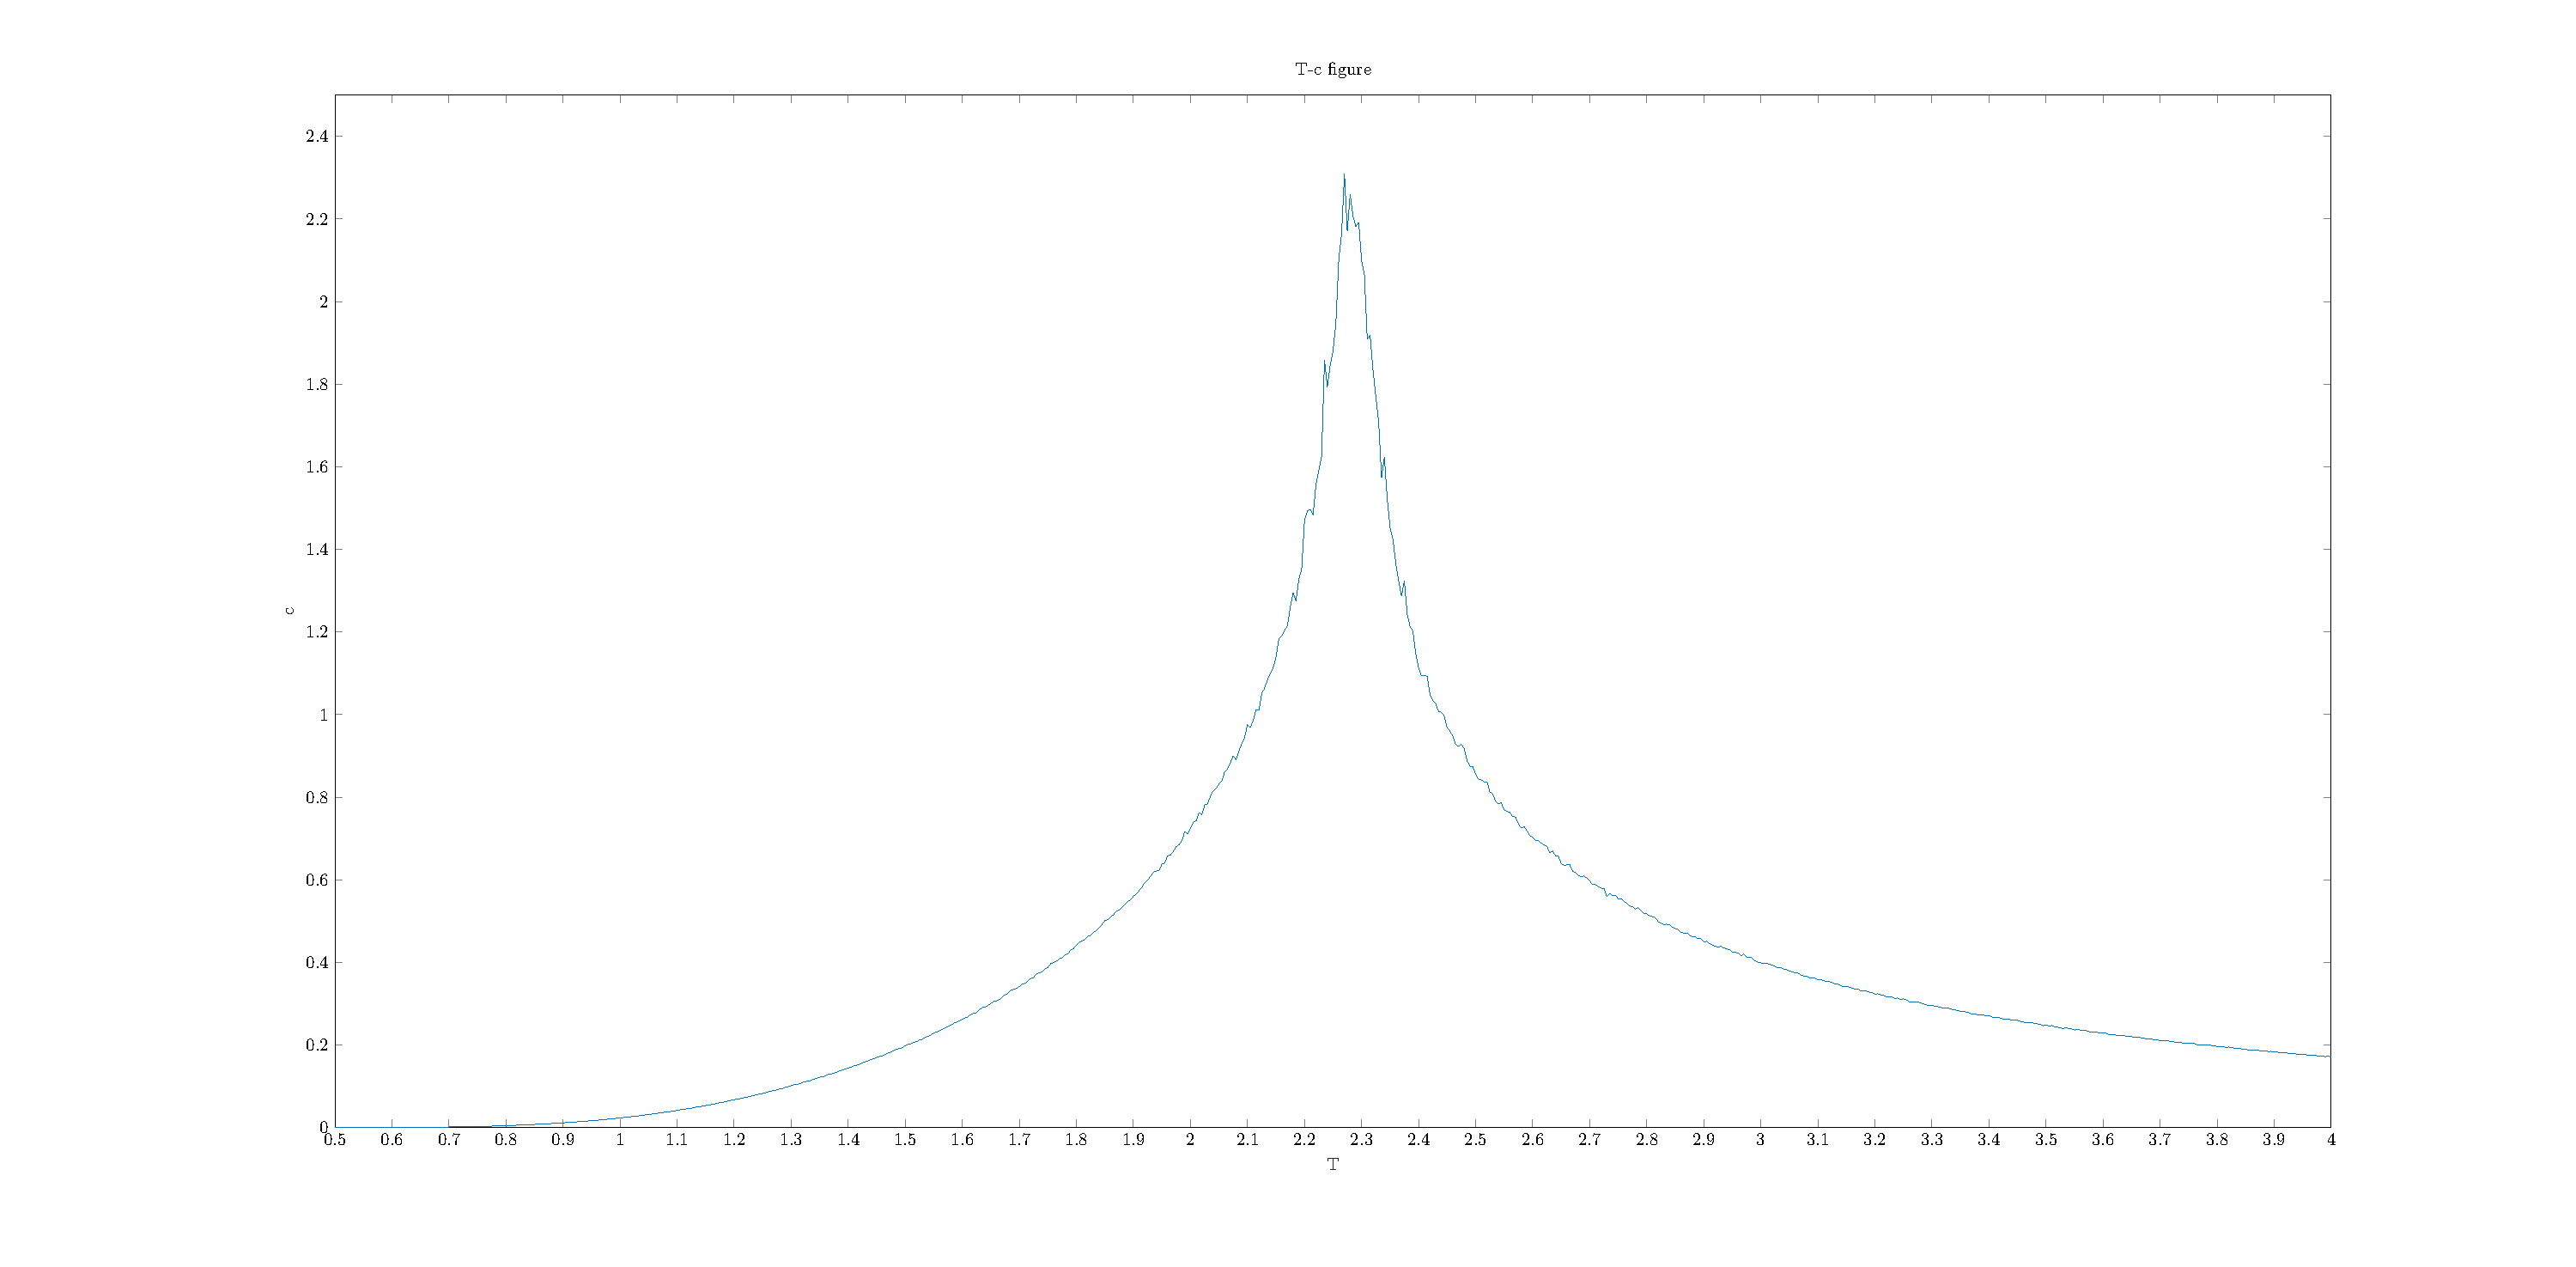
\includegraphics[width=0.8\linewidth]{Tc.pdf}
		\caption{T-c}
	\end{figure}
  
	\begin{figure}\label{fig:Tu}
		\centering
		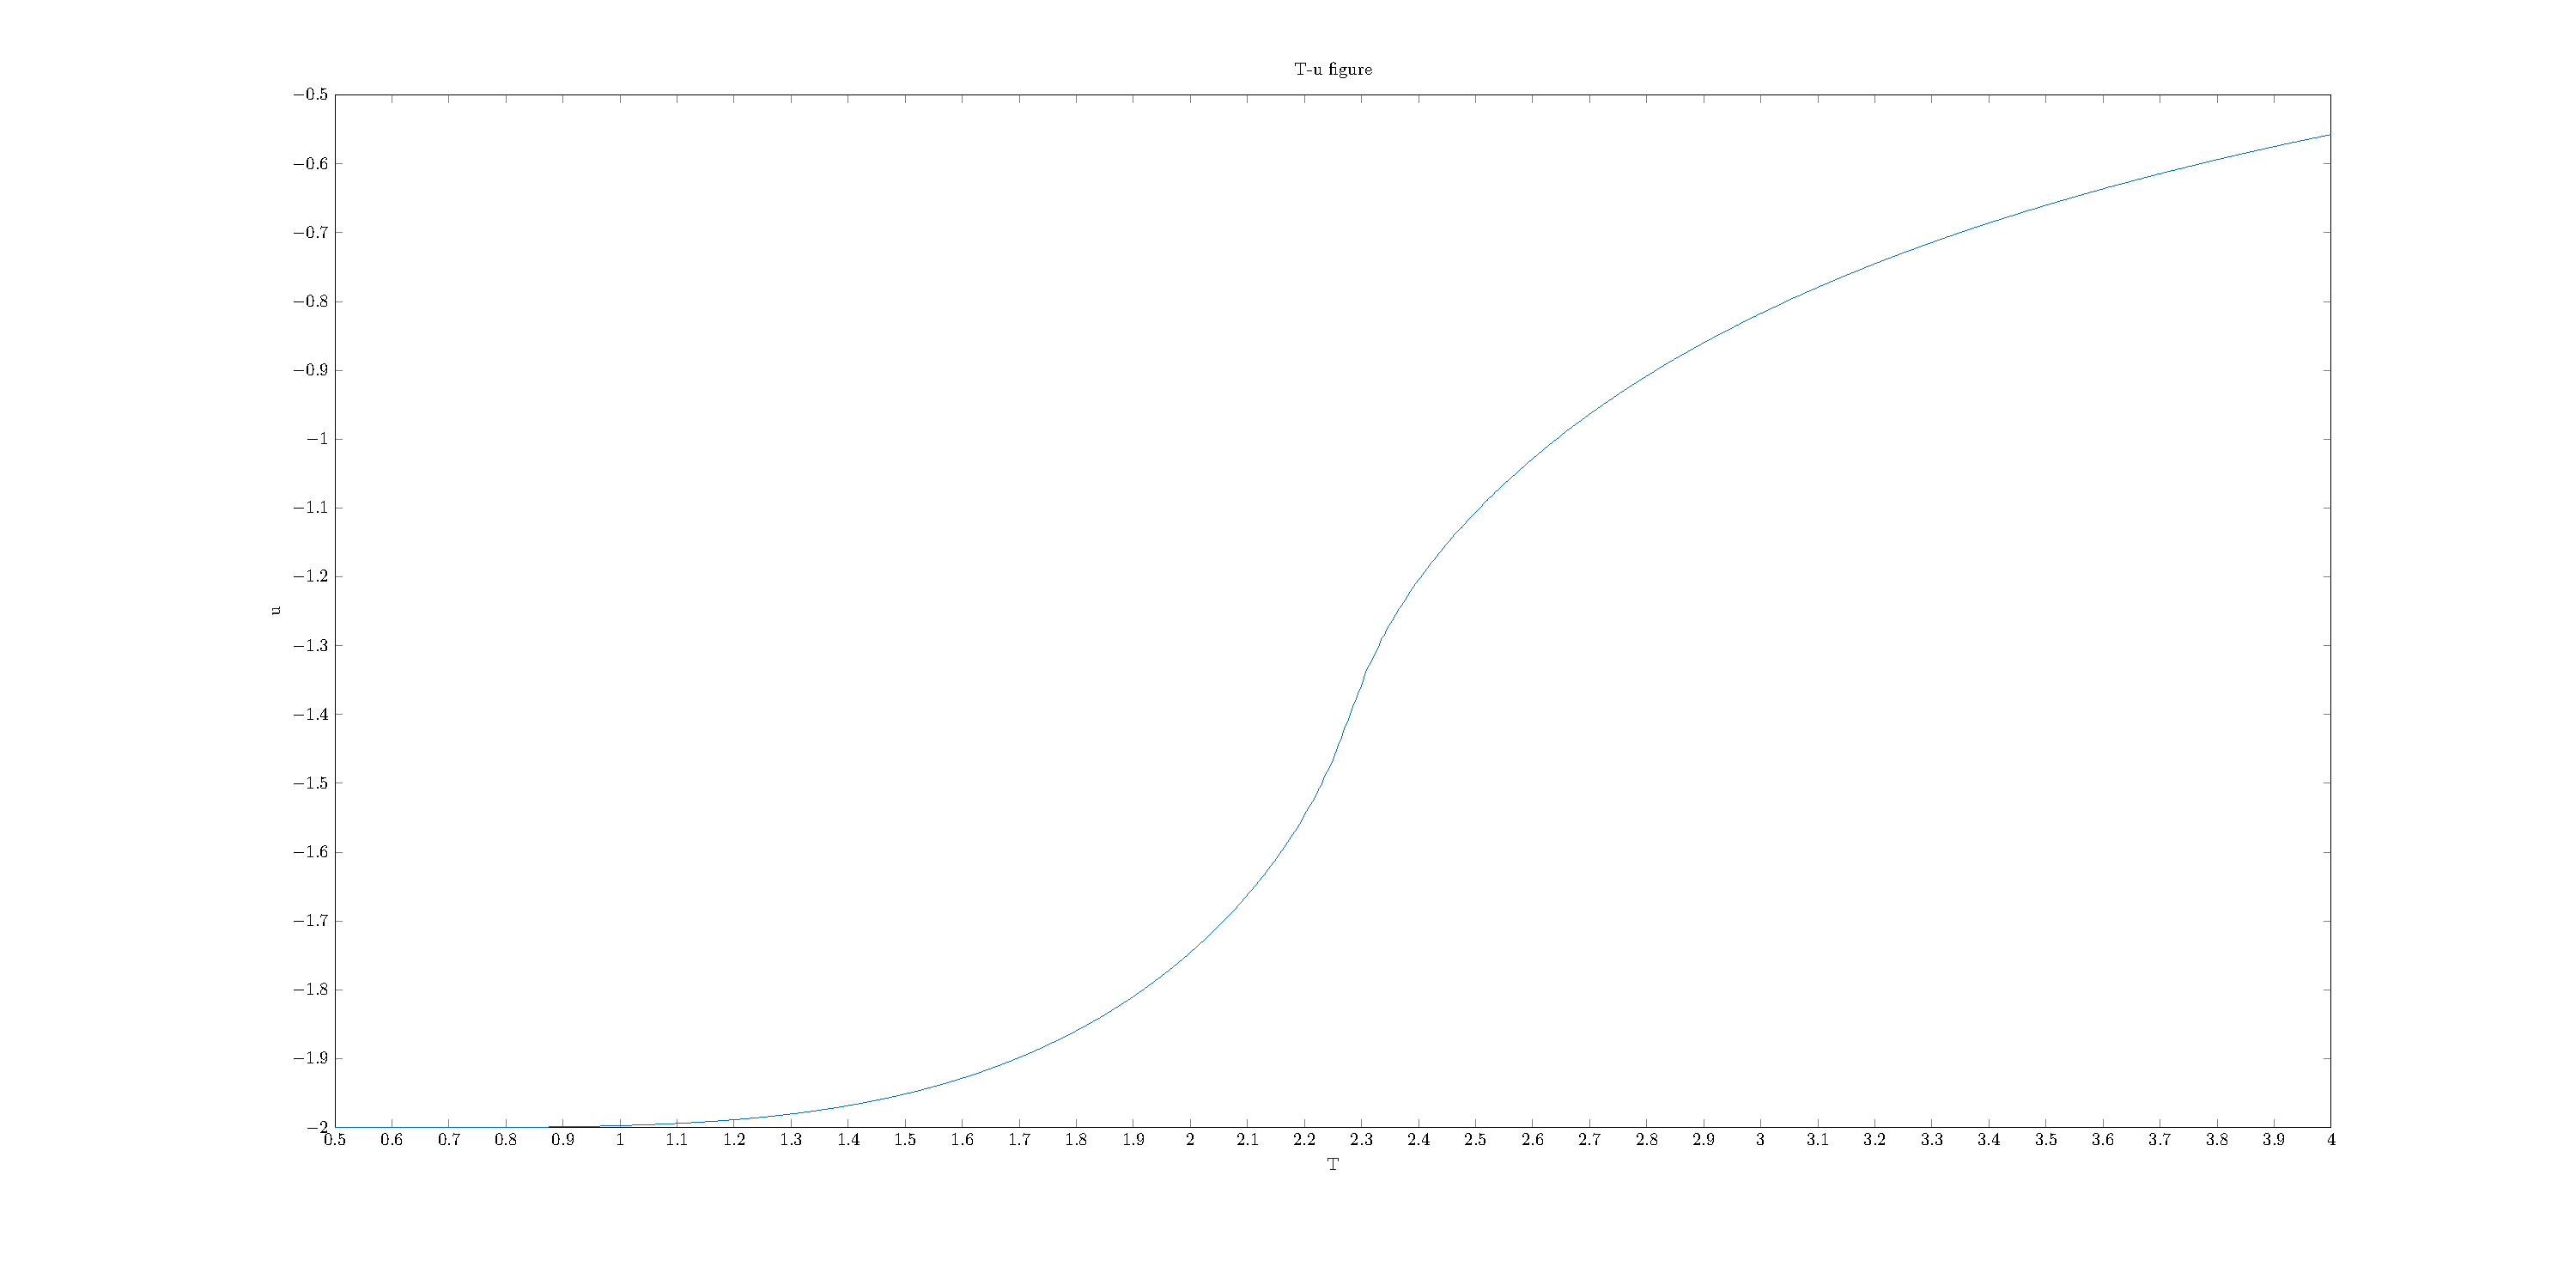
\includegraphics[width=0.8\linewidth]{Tu.pdf}
		\caption{T-u}
	\end{figure}
  \item And in problem 2, we set the size of grid as \(64 \times 64\) and the programing process time as \(1000000\), \(T\) ranges from \(0.5\sim4\) with internal \(0.2\), \(H\) ranges from \(0\sim1\) with internal \(0.1\). 
    We observe from \Cref{fig:THM} that the magnetization \(M\) change near the critical temperature, i. e. \(T_c\).
    When \(T < T_c\), \(m\) will be so close to \(1\), no matter what \(H\) is. When \(T>T_c\), \(m\) is very close to 
    \(0\) in the condition with tiny \(H\), and becomes bigger as \(H\) increases but will near reach \(1\).
    Besides, \(T > T_c\), in the same \(H\), as \(T\) increases, \(m\) decreases.
    We can infer from it that, when \(T\) is low, the magnet has magnetization, when \(T\) increases, the magnet may disappears, which means it has not permanently magnetization.
	\begin{figure}\label{fig:THM}
		\centering
		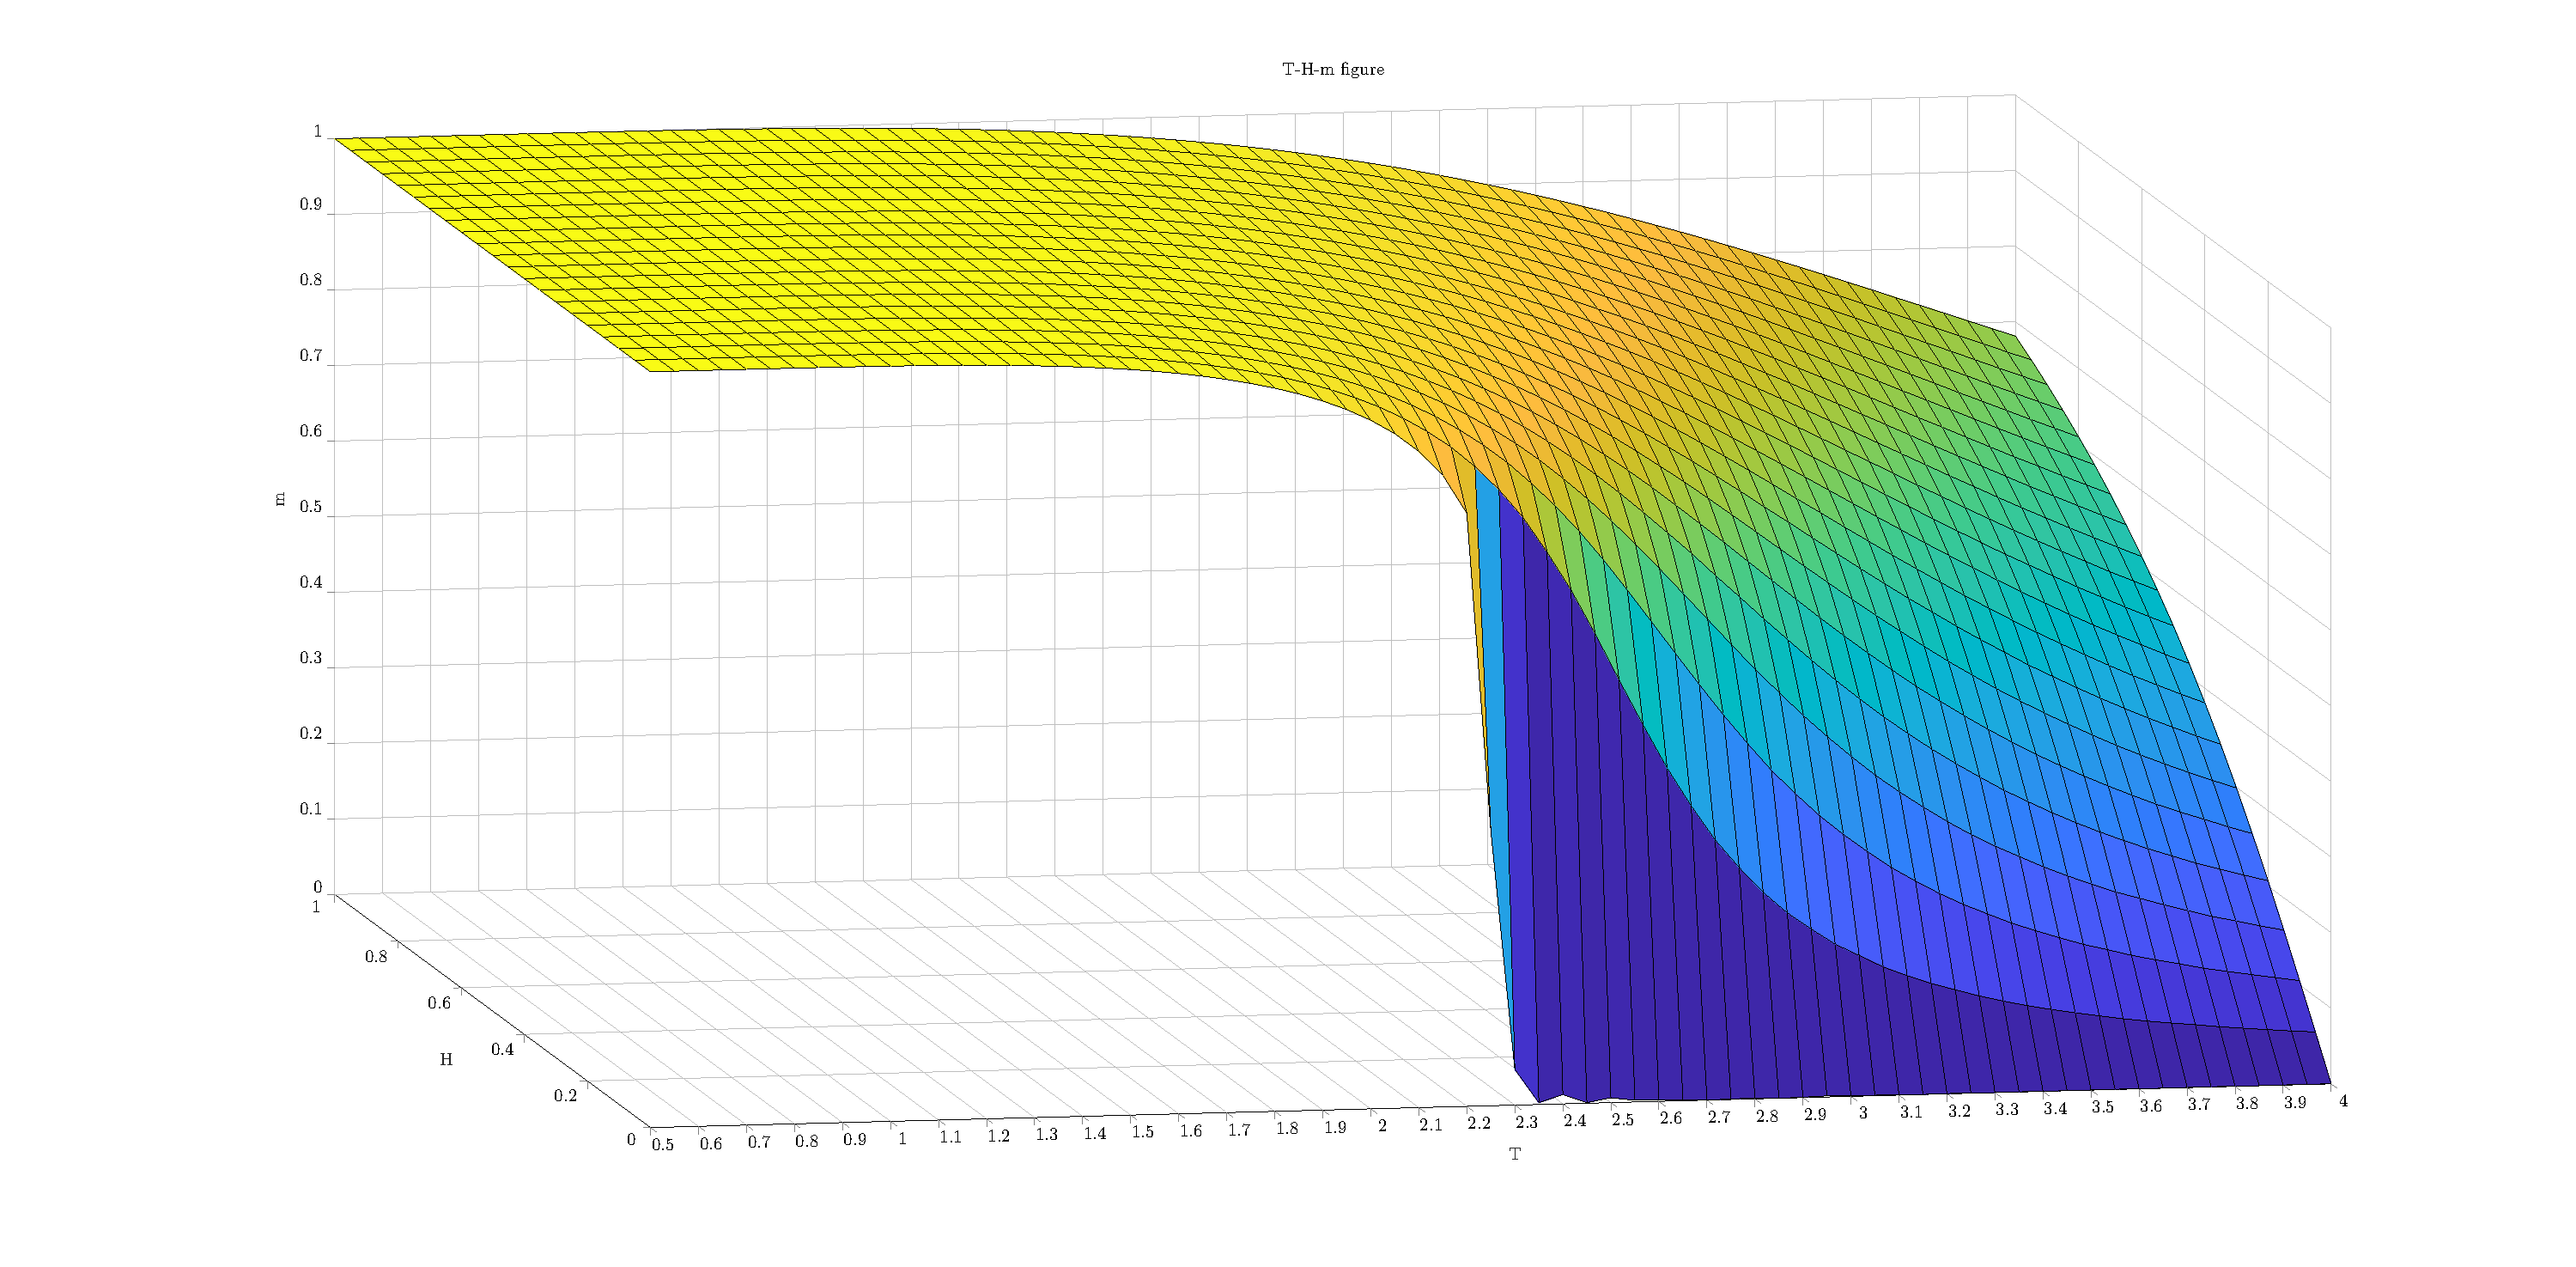
\includegraphics[width=0.8\linewidth]{THM.pdf}
		\caption{T-H-M}
	\end{figure}
\end{enumerate}
\section{The issues you encounter and how you overcome }
First of all, when we was running our program, our compute is not capable enough. But fortunately, 
we have a generous teacher, who borrowed us his compute to complete our program.

\section{ Possible discussion about the results and further thinking }
Ising model can be applied to many other situations and fields. For example, opinion dynamics.
Consider a group of people, each person can support one of two different candidates (like A and B).
The candidate one support may change after exchanging ideas with sourroundings. 
What's more, the residents there may be influenced by advertisement of candidates. This is a typical
reality situation for Ising model.

Besides, we can apply the Ising model to neuroscience. The activity of neuros in the brain can be 
modelled statistically. Each neuron at anytime is either active or inactive. Hopfield suggested in 1982
that a dynamic Ising model would provide a first approximate to a neural network which is capable of learning.
And following the general approach of a lot scientists, we can model the process of neurons by the following 
model. Given a collection of neurons, we assume the energy as:
\begin{equation}
\, E = -1/2 \sum_{ij}J_{ij}SiSj-\sum_i h_iS_i
\end{equation}
In this process, we can apply Ising model to simulate it. 


%\bibliographystyle{plainnat}
%\bibliography{report}

\end{document}                          % The required last line
